\documentclass{beamer}

\usepackage{pgfplots}

\usetheme{Baba}

\title{Real-world applications of Artificial Intelligence in pre-dementia diagnostics and treatment administration}
\date{23.01.2025}
\author{Esten H. Leonardsen}

\definecolor{cases-default}{HTML}{EB5353}
\definecolor{controls-default}{HTML}{0079FF}
\definecolor{healthy-default}{HTML}{36AE7C}
\definecolor{maps}{HTML}{C58940}

\newcommand{\mriside}[4]{
    \def\mridepth{0.75}

    \node[inner sep=0pt] (input) at (#1, #2) {
        \includegraphics[height=#3, width=#3]{#4}
    };

    \draw[fill=black] (input.north west) --
        ($ (input.north west) + (0.5 * \mridepth, 0.5 * \mridepth) $) --
        ($ (input.north east) + (0.5 * \mridepth, 0.5 * \mridepth) $) --
        (input.north east) -- cycle;
    \draw[fill=black] (input.north east) --
        ($ (input.north east) + (0.5 * \mridepth, 0.5 * \mridepth) $) --
        ($ (input.south east) + (0.5 * \mridepth, 0.5 * \mridepth) $) --
        (input.south east) -- cycle;
    \draw[] (input.north west) --
        ($ (input.north west) - (0.5 * \mridepth, 0.5 * \mridepth) $) --
        ($ (input.south west) - (0.5 * \mridepth, 0.5 * \mridepth) $) --
        (input.south west) -- cycle;
    \draw[] (input.north east) --
        ($ (input.north east) - (0.5 * \mridepth, 0.5 * \mridepth) $) --
        ($ (input.south east) - (0.5 * \mridepth, 0.5 * \mridepth) $) --
        (input.south east) -- cycle;
    \draw[] ($ (input.north west) - (0.5 * \mridepth, 0.5 * \mridepth) $) --
        ($ (input.north east) - (0.5 * \mridepth, 0.5 * \mridepth) $);
    \draw[] ($ (input.south west) - (0.5 * \mridepth, 0.5 * \mridepth) $) --
        ($ (input.south east) - (0.5 * \mridepth, 0.5 * \mridepth) $);
}


\newcommand{\inputside}[3]{
    \mriside{#1}{#2}{#3}{data/mri_sagittal.png}
}

\newcommand{\convside}[6]{
    \def\sidex{#1}
    \def\sidey{#2}
    \def\sidewidth{#3}
    \def\sideheight{#4}
    \def\sidefillcolour{#5}
    \def\sidename{#6}

    \node[
        fill=\sidefillcolour,
        inner sep=0pt,
        outer sep=0pt,
        minimum width=\sidewidth,
        minimum height=\sideheight,
        draw=black
    ] (\sidename) at (\sidex, \sidey) {};
}

\newcommand{\convtop}[4]{
    \def\topbase{#1}
    \def\topwidth{#2}
    \def\topheight{#3}
    \def\topfillcolour{#4}

    \draw[fill=\topfillcolour,draw=black] #1 --
        ($ #1 + (#3, #3) $) --
        ($ #1 + (#3+#2, #3) $) --
        ($ #1 + (#2, 0) $);
}

\newcommand{\convfront}[3]{
    \def\frontbase{#1}
    \def\frontsize{#2}
    \def\frontfillcolour{#3}

    \draw[black, fill=\frontfillcolour] #1 --
        ($ #1 + (1*#2, 1*#2) $) --
        ($ #1 + (1*#2, 1*#2 - 2*#2) $) --
        ($ #1 + (0, -2*#2) $);
}

\newcommand{\convchannel}[7]{
    \def\channelx{#1}
    \def\channely{#2}
    \def\channelnodedepth{#3}
    \def\channelnodesize{#4}
    \def\channelnodecount{#5}
    \def\channelcolour{#6}
    \def\includefront{#7}

    \def\huemin{20}
    \def\huemax{80}

    \pgfmathsetmacro{\iterations}{#5-1}
    \foreach \i in {0,...,\iterations} {
        \pgfmathsetmacro{\hue}{int(random(\huemin, \huemax))}
        \convside{#1}{#2+\i*-#4}{#3 cm}{#4 cm}{#6!\hue}{n\i0}

        \foreach \j in {0,...,\iterations} {
            \pgfmathsetmacro{\innerhue}{int(random(\huemin, \huemax))}
            \ifnum\j=0
                \pgfmathsetmacro{\innerhue}{\hue}
            \fi

            \ifnum\includefront=1
                \convfront{($ (n00.north east) + (0.5*\j*#4, 0.5*\j*#4 - \i*#4) $)}{0.5*#4}{#6!\innerhue}
            \fi

            \ifnum\i=0
                \convtop{($ (n\i0.north west) + (0.5*\j*#4, 0.5*\j*#4) $)}{#3}{0.5*#4}{#6!\innerhue}
            \fi
        }
    }
}
\newcommand{\convlayer}[7]{
    \def\layerx{#1}
    \def\layery{#2}
    \def\layernodedepth{#3}
    \def\layernodesize{#4}
    \def\layernodecount{#5}
    \def\layerdepth{#6}
    \def\layercolour{#7}

    \pgfmathsetmacro{\layeriterations}{\layerdepth-1}
    \foreach \i in {0,...,\layeriterations}{
        \pgfmathsetmacro{\x}{\layerx + \i * \layernodedepth}
        \pgfmathsetmacro{\islast}{\i == \layeriterations ? 1 : 0}
        \convchannel{\x}{\layery}{\layernodedepth}{\layernodesize}{\layernodecount}{\layercolour}{\islast}
    }
}

\newcommand{\modelarrow}[5]{
    \begin{scope}[transparency group, opacity=0.5]
        \draw[-stealth, line width=2pt, #3] #1 to [in=#4, out=#5] #2;
    \end{scope}
}

\newcommand{\cnnarrow}[3]{
    \modelarrow{#1}{#2}{#3}{180}{0}
}

\newcommand{\cnn}[6]{
    \def\xmin{#1}
    \def\ymin{#2}
    \def\nodedepth{#3}
    \def\nodesize{#4}
    \def\modelcolour{#5}
    \def\annotate{#6}

    \convlayer{#1 - 0.06 + 0.4}{#2 + 2.5 * #4}{#3}{#4}{12}{3}{\modelcolour}
    \cnnarrow{(#1 + 0.95, #2)}{(#1+2.2, #2)}{#5}

    \convlayer{#1 + 1.44 + 0.4}{#2 + 1.5 * #4}{#3}{#4}{8}{5}{\modelcolour}
    \cnnarrow{(#1 + 2.43, #2)}{(#1+3.5, #2)}{#5}

    \convlayer{#1 + 2.77 + 0.4}{#2 + 0.5 * #4}{#3}{#4}{4}{7}{\modelcolour}
    \cnnarrow{(#1 + 3.75, #2)}{(#1+5, #2)}{#5}

    \convlayer{#1 + 3.93 + 0.4}{#2 + 0}{#3}{#4}{2}{9}{\modelcolour}

    \ifdim #6 pt = 1 pt
        \draw[thick, dashed] (#1 + 0.22, #2 + 1.43) --
                            (#1 + 5.13, #2 + 1.43) --
                            (#1 + 5.13, #2 - 1.42) --
                            (#1 + 0.22, #2 - 1.42) -- cycle;
        \node[anchor=south, text depth=0, font=\scriptsize\selectfont] at (#1 + 2.675, #2 + 1.43) {
            \textbf{Convolutional Neural Network}
        };
    \fi
}

\newcommand{\prognostic}{
    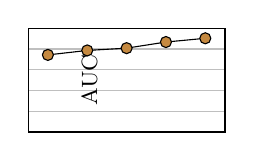
\begin{tikzpicture}
        \begin{axis}[
            height=2.9cm,
            width=4.08cm,
            xmajorticks=false,
            xmin=0.5,
            xmax=5.5,
            ymin=0,
            ymax=1,
            ylabel=\footnotesize{AUC},
            ymajorticks=false,
            ymajorgrids=true,
            y label style={at={(axis description cs:0.4,.5)}}
        ]

            \addplot[mark=*, draw=black, mark options={fill=maps}] coordinates {
                (1, 0.743)
                (2, 0.786)
                (3, 0.808)
                (4, 0.867)
                (5, 0.903)
            };
        \end{axis}
    \end{tikzpicture}
}

\newsavebox{\prognosticaucs}
\sbox{\prognosticaucs}{
    \prognostic
}

\newcommand{\mciconcept}[1]{
    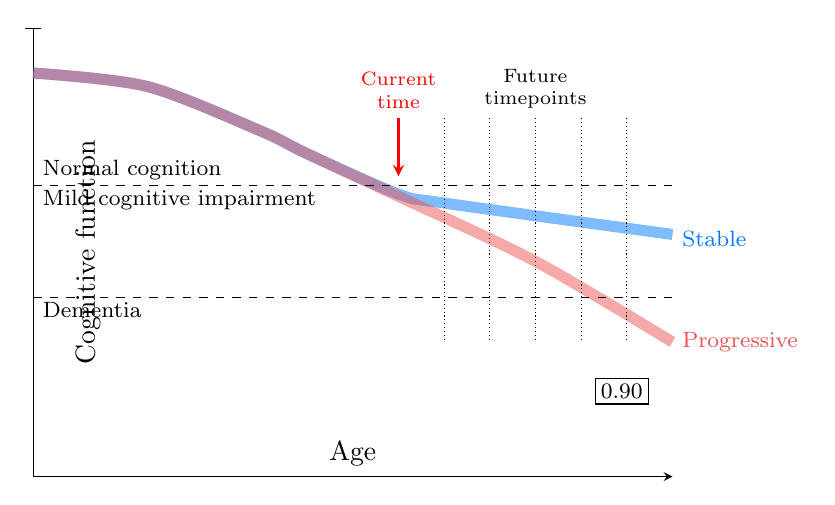
\begin{tikzpicture}
        \begin{axis}[
            height=0.6\textwidth,
            width=0.8\textwidth,
            xlabel={Age},
            ylabel={Cognitive function},
            ticks=none,
            axis x line=bottom,
            axis y line=left,
            y axis line style={-|},
            xmin=0,
            xmax=1.4,
            ymin=0,
            ymax=1,
            clip=false,
            y label style={at={(axis description cs:0.12,0.5)}},
            x label style={at={(axis description cs:0.5,0.1)}}
        ]
            \addplot[draw=controls-default, smooth, line width=4pt, opacity=0.5] coordinates {
                (0, 0.9)
                (0.25, 0.87)
                (0.5, 0.77)
                (0.6, 0.72)
                (0.8, 0.63)
                (0.9, 0.61)
                (1.4, 0.54)
            };
            \addplot[draw=cases-default, smooth, line width=4pt, opacity=0.5] coordinates {
                (0, 0.9)
                (0.25, 0.87)
                (0.5, 0.77)
                (0.6, 0.72)
                (0.8, 0.625)
                (1.1, 0.48)
                (1.4, 0.3)
            };
            \addplot[dashed] coordinates {
                (0, 0.65)
                (1.4, 0.65)
            };
            \addplot[dashed] coordinates {
                (0, 0.4)
                (1.4, 0.4)
            };
            \node[anchor=south west] at (axis cs: 0, 0.64) {\footnotesize{Normal cognition}};
            \node[anchor=north west] at (axis cs: 0, 0.66) {\footnotesize{Mild cognitive impairment}};
            \node[anchor=north west] at (axis cs: 0, 0.41) {\footnotesize{Dementia}};

            \node[anchor=west] at (axis cs: 1.4, 0.53) {\textcolor{controls-default}{\footnotesize{Stable}}};
            \node[anchor=west] at (axis cs: 1.4, 0.3) {\textcolor{cases-default}{\footnotesize{Progressive}}};

            \draw[-stealth, red, thick] (axis cs: 0.8, 0.8) -- (axis cs: 0.8, 0.67);
            \node[anchor=south, font=\scriptsize, text=red, align=center] at (axis cs: 0.8, 0.8) {Current\\time};

            \draw[densely dotted] (axis cs: 0.9, 0.8) -- (axis cs: 0.9, 0.3);
            \draw[densely dotted] (axis cs: 1, 0.8) -- (axis cs: 1, 0.3);
            \draw[densely dotted] (axis cs: 1.1, 0.8) -- (axis cs: 1.1, 0.3);
            \draw[densely dotted] (axis cs: 1.2, 0.8) -- (axis cs: 1.2, 0.3);
            \draw[densely dotted] (axis cs: 1.3, 0.8) -- (axis cs: 1.3, 0.3);

            \node[anchor=south, align=center, font=\scriptsize] at (axis cs: 1.1, 0.8) {Future\\timepoints};

            \node[] at (axis cs: 1.045, 0.155) {
                \usebox{\prognosticaucs}
            };
            \node[anchor=west, draw=black, fill=white, inner sep=2pt] at (axis cs: 1.23, 0.19) {\footnotesize{0.90}};

        \end{axis}
    \end{tikzpicture}
}

\newsavebox{\mciheatmaps}
\sbox{\mciheatmaps}{
    \mciconcept{6}
}

\begin{document}
    \begin{frame}
        \titlepage
    \end{frame}

    \begin{frame}{Background}
        \centering
        \begin{tikzpicture}

            \visible<1>{
                \node[] at (-5.05, 0) {};
                \node[] at (5.05, 0) {};

                \inputside{-3.95}{0}{1.5cm}
                \cnnarrow{(input.east)}{($ (input.center) + (2, 0) $)}{black}
                \node[
                    font=\scriptsize\linespread{0.9}\selectfont,
                    align=left,
                    anchor=west
                ] (output) at (2.95, 0) {
                    Diagnostic\\status
                };
                \cnn{-2.55}{0}{0.066}{0.15}{black}{1}
                \cnnarrow{($ (output.west) - (0.54, 0) $)}{($ (output.west) + (0.1, 0) $)}{black}
            }
            \visible<2>{
                \node[] at (0, 0) {
                    \usebox{\mciheatmaps}
                };
            }
            \visible<3>{
                \node[draw=black, fill=white, inner sep=0pt] (paper1) at (0, 1.35) {
                    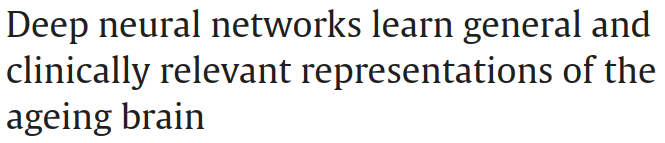
\includegraphics[width=8cm]{data/paper1.png}
                };
                \draw[red, thick] ($ (paper1.west) + (0.1, -0.25) $)-- ($ (paper1.west) + (3.5, -0.25) $);
                \node[text width=8cm, align=center, anchor=north, font=\tiny] at (paper1.south) {
                    \textit{Deep neural networks learn general and clinically relevant representations of the ageing brain}, Leonardsen et al., 2022. NeuroImage, 256, 119210
                };

                \node[draw=black, fill=white, inner sep=0pt] (paper3) at (0, -1.35) {
                    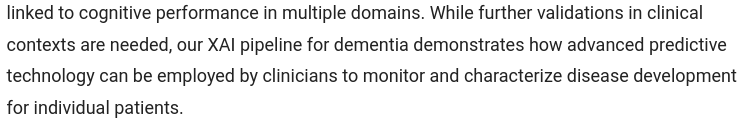
\includegraphics[width=8cm]{data/paper3.png}
                };
                \draw[red, thick] ($ (paper3.west) + (1.72, -0.28) $)-- ($ (paper3.west) + (3.63, -0.28) $);
                \node[fill=white, opacity=0.75, anchor=north west, minimum width=8cm, minimum height=0.3cm] at (paper3.north west) {};
                \node[text width=8cm, anchor=north] at (paper1.south) {};
                \node[fill=white, opacity=0.75, anchor=north west, minimum width=1.9cm, minimum height=0.3cm] at ($ (paper3.north west) - (0, 0.3) $) {};
                \node[text width=8.4cm, align=center, anchor=north, font=\tiny] at (paper3.south) {
                    \textit{Constructing personalized characterizations of structural brain aberrations}\\ \textit{in patients with dementia using explainable artificial intelligence},\\ Leonardsen et al., 2024.  npj Digital Medicine, 7(1), 110
                };
            }
            \visible<4>{
                \node[inner sep=0pt, draw=black, label=below:\tiny{https://github.com/estenhl/pyment-public}] (git) at (0, 0) {
                    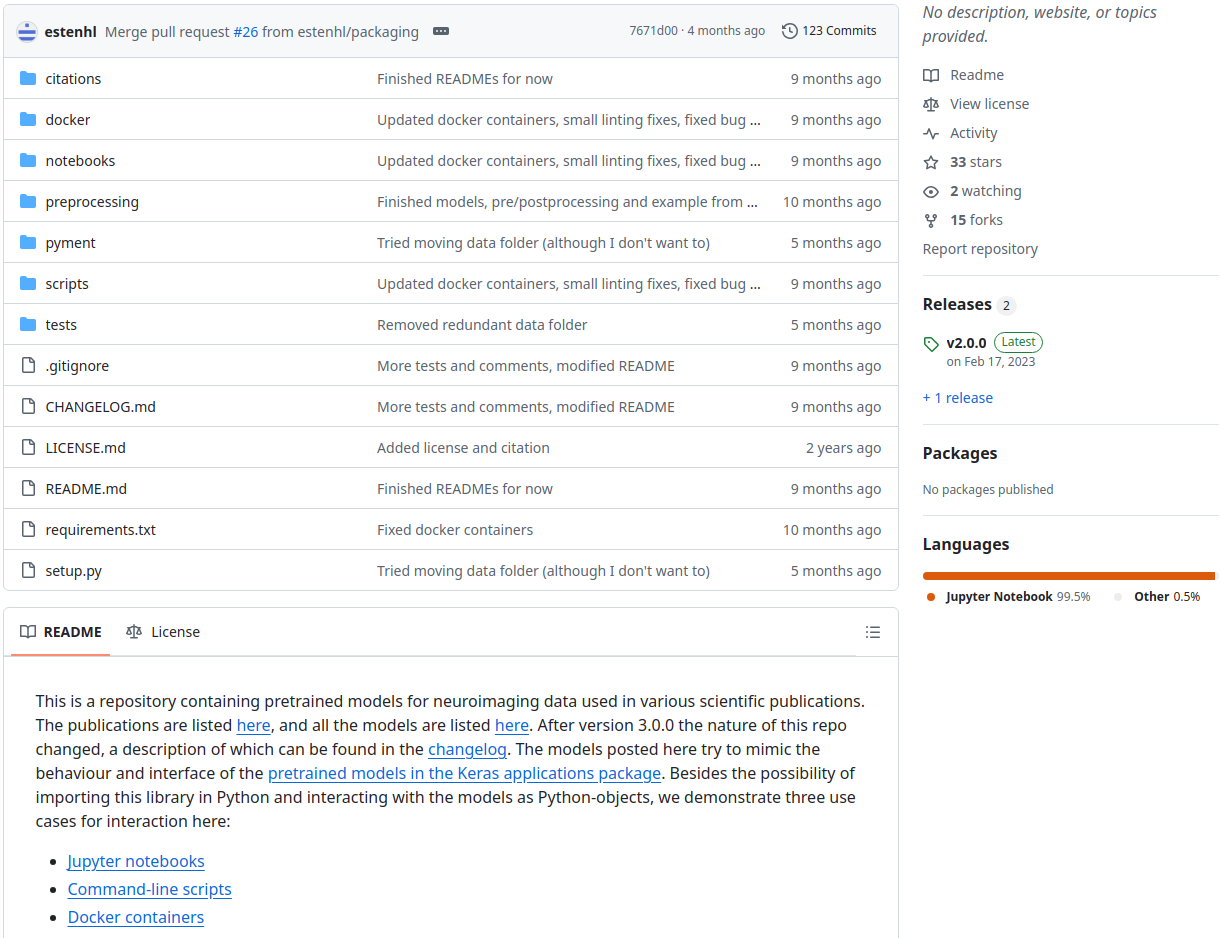
\includegraphics[width=9cm]{data/github.png}
                };
            }
            \visible<5-6>{
                \node[text width=10cm, font=\small] at (0, 0) {
                    \begin{enumerate}
                        \item Showcase the \textbf{general efficacy} of artificial intelligence for demonstrative clinical use-cases
                        \item<6> Build predictive models to solve specific \textbf{real-world clinical problems} using \textbf{commercially available data}
                        \item<6> Ensure the \textbf{robustness and utility} of the models through extensive validation
                        \item<6> Collaborate with clinicians to package the models in \textbf{user-friendly interfaces} integrating smoothly into \textbf{standardized clinical workflows}
                    \end{enumerate}
                };
            }
            \visible<7-8>{
                \node[label={[align=center, font=\scriptsize\linespread{0.9}\selectfont]below:{\textbf{Per Wessel Nore}\\CEO baba.vision}}] at (-3.5, 0) {
                    
\includegraphics[width=2cm]{data/per.png}
                };
            }
            \visible<8>{
                \node[inner sep=0pt, draw=black] at (1.5, 0) {
                    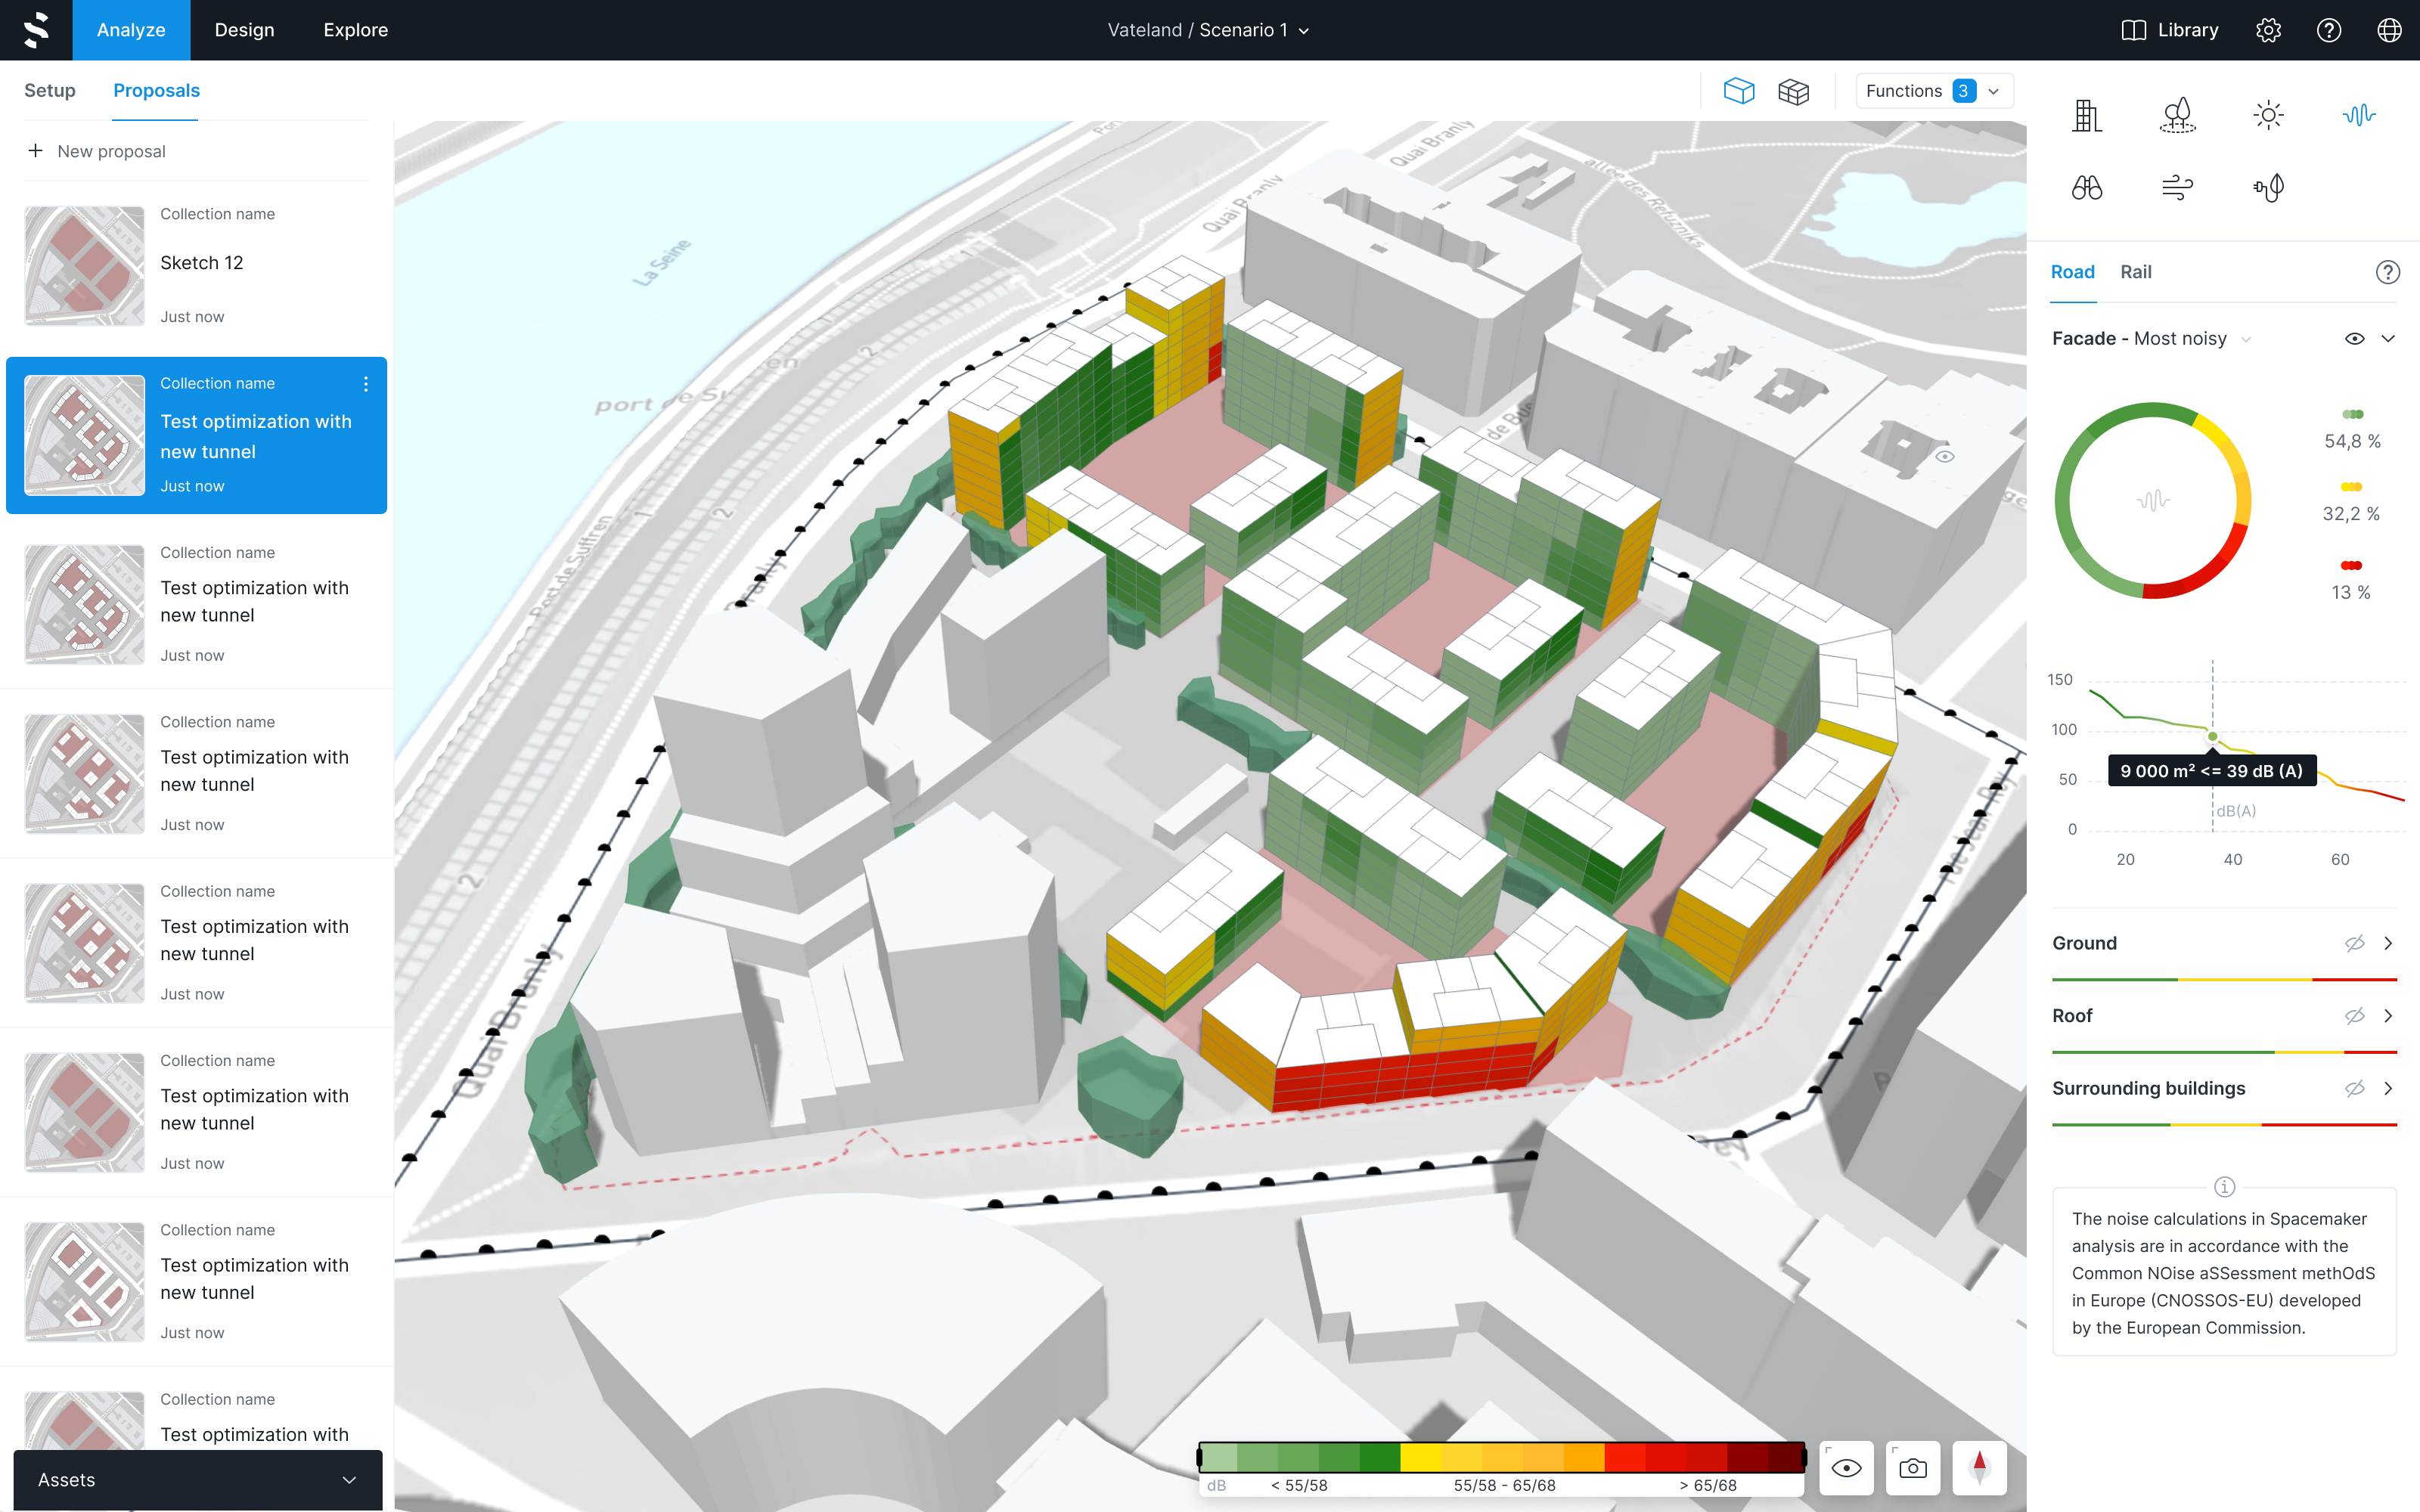
\includegraphics[width=6cm]{data/spacemaker.jpg}
                };
            }
        \end{tikzpicture}
    \end{frame}

    \section{Decision support for neuroradiological examinations in dementia pre-diagnostics}

    \begin{frame}{Neuroradiological decision support}
        \centering
        \begin{tikzpicture}
            \node[] at (0, 4.15) {};
            \node[] at (0, -4.15) {};

            \visible<1>{
                \node[fill=white, draw=black] at (0, 0) {
                    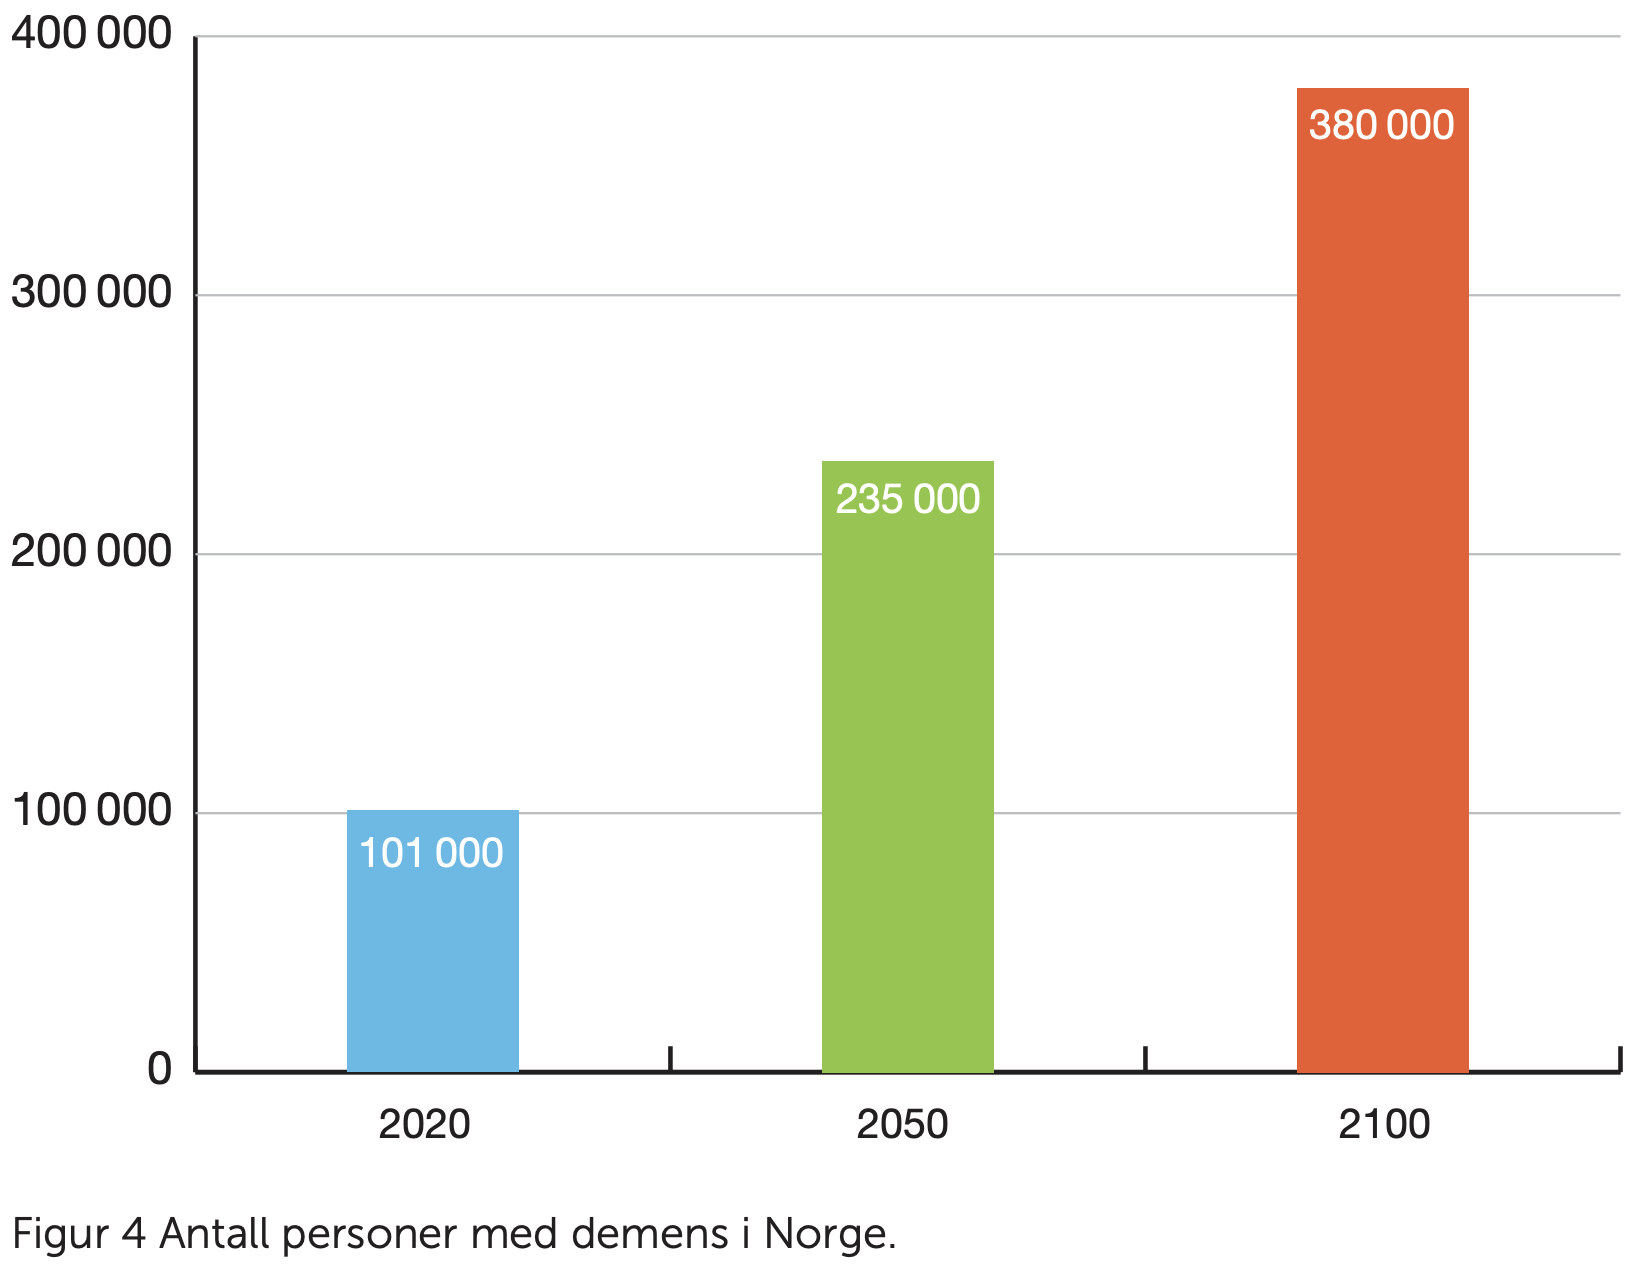
\includegraphics[width=7cm]{data/prevalence.png}
                };
                \node[anchor=south, font=\tiny\linespread{0.9}\selectfont, text width=10.5cm, align=center] at (0, -4.15) {
                    Gjøra L., Kjelvik G. , Strand B.H., Kvello-Alme M., Selbæk G. Forekomst av demens\\i Norge. Rapport Aldring og helse 2020. ISBN: 978-82-8061-579-4
                };
            }
            \visible<2>{
                \node[] at (0, 1) {
                    
\includegraphics[width=5cm]{data/clock.png}
                };

                \node[anchor=south, font=\footnotesize\linespread{0.9}\selectfont, text width=11cm, align=flush center] at (0, -3) {
                    "However, in practice, this [referral for neuroimaging] concerns a very small number of patients, judiciously selected, as to not overwhelm the radiology services which was commented upon as being \textit{\textbf{exceptionally limited and often available off-site in another larger regional hospital}}."
                };

                \node[anchor=south, font=\tiny\linespread{0.9}\selectfont, text width=10.5cm, align=flush center] at (0, -4.15) {
                    Griffanti, L., Serres, F., Cini, L., Walsh, J., Hanayik, T., Pervaiz, U., ... \& Bajre, M. (2024). Brain magnetic resonance imaging software to support dementia diagnosis in routine clinical practice: a barrier to adoption study in the National Health Service (NHS) England. \textit{preprint at medRxiv}, 2024-08.
                };
            }
            \visible<3>{
                \node[ampersand replacement=\&] at (0, 0) {
                    \begin{tabular}{c|c c c c c}
                        &1&2&3&4&5\\
                        \hline
                        1&38&273&17&4&0\\
                        2&0&92&144&12&0\\
                        3&0&6&89&31&2\\
                        4&0&0&3&19&5\\
                        5&0&0&0&0&5\\
                    \end{tabular}
                };

                \node[anchor=south, font=\tiny\linespread{0.9}\selectfont, text width=10.5cm, align=center] at (0, -4.15) {
                    Mårtensson, G., Håkansson, C., Pereira, J. B., Palmqvist, S., Hansson, O., van Westen, D., \& Westman, E. (2020). Medial temporal atrophy in preclinical dementia: visual and automated assessment during six year follow-up. \textit{NeuroImage: Clinical}, \textit{27}, 102310.
                };
            }
            \visible<4>{
                \node[inner sep=0pt, draw=black] (prototype) at (0, 0) {
                    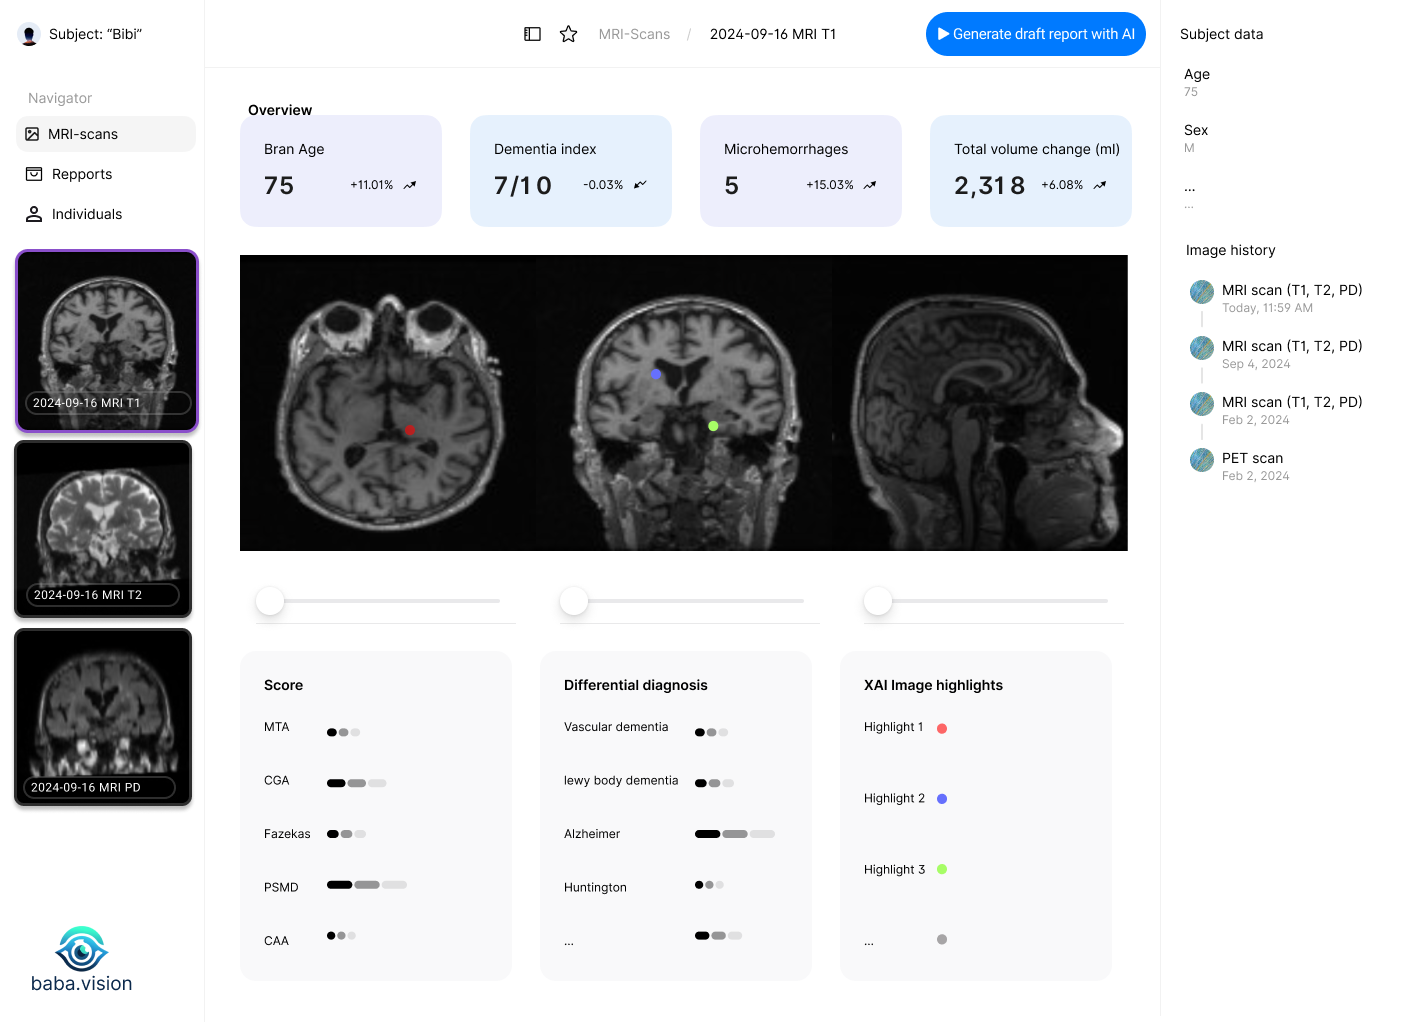
\includegraphics[width=9cm]{data/prototype.png}
                };
            }
        \end{tikzpicture}
    \end{frame}

    \section{Treatment response prediction and monitoring of patients on anti-amyloid therapies}

    \newcommand{\responseplot}[1]{
        \begin{tikzpicture}
            \begin{axis}[
                height=6cm,
                width=9cm,
                axis lines=left,
                xmajorticks=false,
                ymajorticks=false,
                xlabel={Time},
                ylabel={Predicted ARIA risk},
                xmin=0,
                xmax=1,
                ymin=0,
                ymax=1,
                clip=false
            ]
                \draw[dashed] (axis cs: 0.2, -0.05) -- (axis cs: 0.2, 1.05);
                \node[anchor=south, font=\footnotesize\linespread{0.9}\selectfont, align=center, inner sep=2pt] at (axis cs: 0.2, 1.05) {First\\treatment};
                \draw[densely dotted, red] (axis cs: 0, 0.6) -- (axis cs: 1, 0.6);
                \node[text=red, font=\footnotesize, anchor=south east, inner sep=2pt] at (axis cs: 1, 0.6) {
                    Acceptable risk
                };

                \ifnum#1 = 0
                    \addplot[only marks, mark=*, teal, mark size=3pt] coordinates {
                        (0.2, 0.75)
                    };
                \fi


                \ifnum#1 = 1
                    \addplot[mark=*, teal, mark size=3pt, smooth] coordinates {
                        (0.2, 0.75)
                        (0.4, 0.7)
                        (0.6, 0.6)
                    };
                \fi

            \end{axis}
        \end{tikzpicture}
    }

    \newsavebox{\responseprediction}
    \sbox{\responseprediction}{
        \responseplot{0}
    }

    \newsavebox{\responsetrajectory}
    \sbox{\responsetrajectory}{
        \responseplot{1}
    }
    \newcommand{\nnneuron}[3]{
        \node[circle, minimum size=0.3cm, inner sep=0pt, draw=none, fill=#3, draw=#3] (#2) at #1 {};
    }
    \newcommand{\neuronconnection}[4]{
        \begin{scope}[transparency group, opacity=0.5]
            \draw[#4,line width=1.5pt, #3] (#1) to [in=180, out=0] (#2);
        \end{scope}
    }

    \begin{frame}{Treatment response and monitoring}
        \centering
        \begin{tikzpicture}
            \node[] at (0, 4.15) {};
            \node[] at (0, -4.15) {};

            \visible<1>{
                \node[inner sep=0pt, draw=black] at (0, 0) {
                    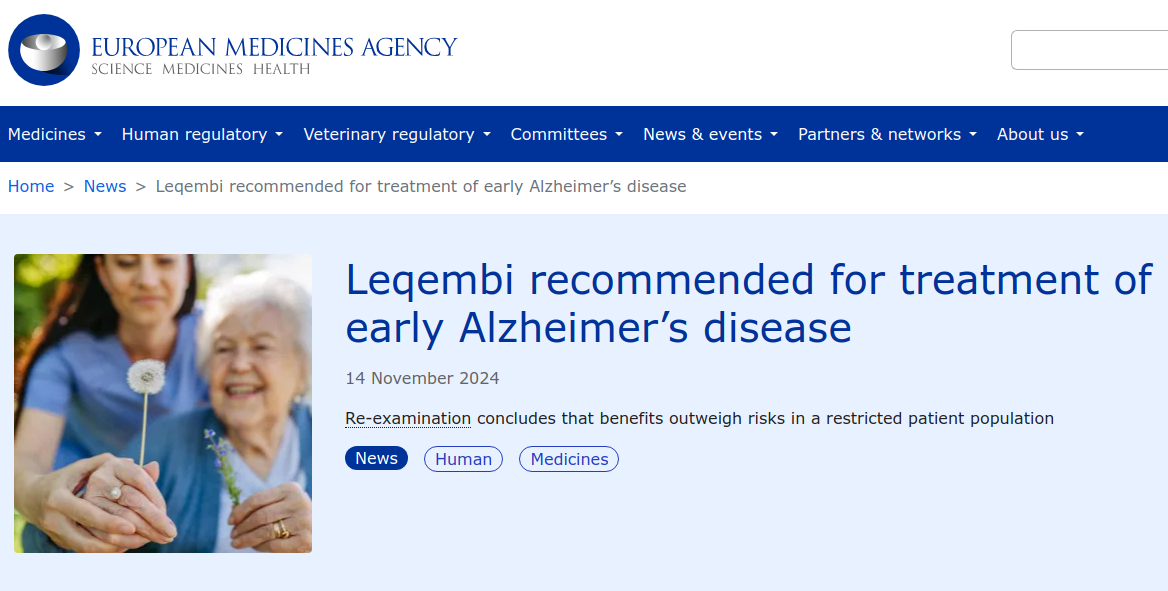
\includegraphics[width=9cm]{data/leqembi_ema.png}
                };
            }
            \visible<2>{
                \node[inner sep=0pt, draw=black] at (0, 0) {
                    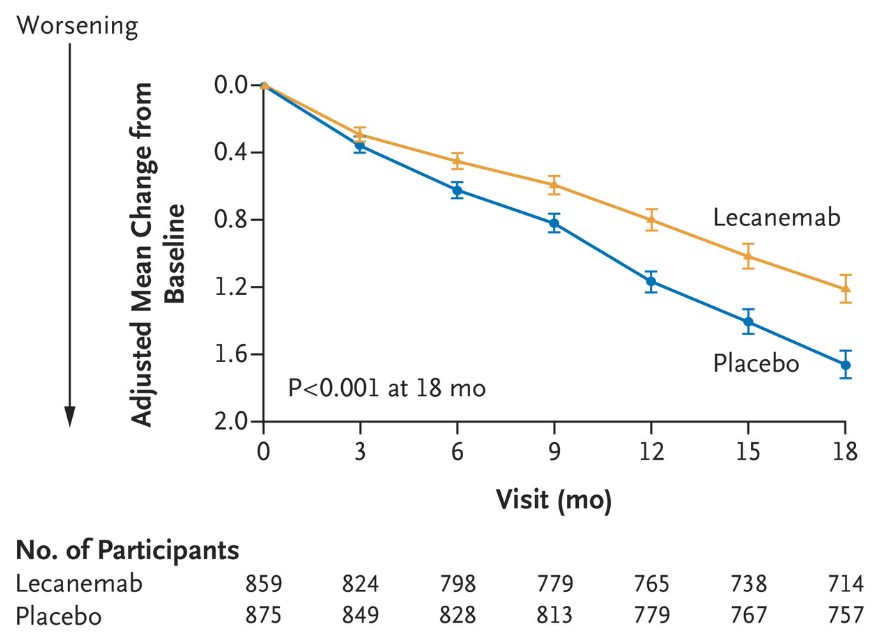
\includegraphics[width=7cm]{data/lecanemab.png}
                };

                \node[anchor=south, font=\tiny\linespread{0.9}\selectfont, text width=10.5cm, align=center] at (0, -4.15) {
                    Van Dyck, C. H., Swanson, C. J., Aisen, P., Bateman, R. J., Chen, C., Gee, M., ... \& Iwatsubo, T. (2023). Lecanemab in early Alzheimer’s disease. \textit{New England Journal of Medicine}, \textit{388}(1), 9-21.
                };
            }
            \visible<3>{
                \node[] at (0, 0) {
                    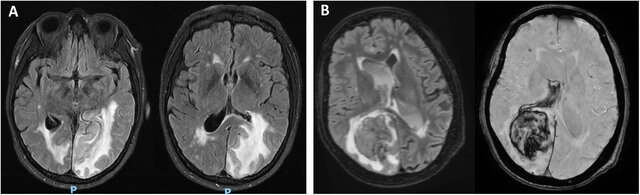
\includegraphics[width=10cm]{data/aria.jpg}
                };
                \node[anchor=south, font=\tiny\linespread{0.9}\selectfont, text width=10.5cm, align=center] at (0, -4.15) {
                    Villain, N., Planche, V., \& Levy, R. (2022). High-clearance anti-amyloid immunotherapies\\in Alzheimer's disease. Part 1: Meta-analysis and review of efficacy and safety data, and medico-economical aspects. \textit{Revue neurologique}, \textit{178}(10), 1011-1030.
                };
            }
            \visible<4-5>{
                \node[anchor=south, font=\tiny\linespread{0.9}\selectfont, text width=10.5cm, align=center] at (0, -4.15) {
                    Honig, L. S., Barakos, J., Dhadda, S., Kanekiyo, M., Reyderman, L., Irizarry, M., ... \& Sabbagh, M. (2023). ARIA in patients treated with lecanemab (BAN2401) in a phase 2 study in early Alzheimer's disease.\\\textit{Alzheimer's \& Dementia: Translational Research \& Clinical Interventions}, \textit{9}(1), e12377.
                };
            }
            \visible<4>{
                \node[draw=black, inner sep=0pt] at (0, 0) {
                    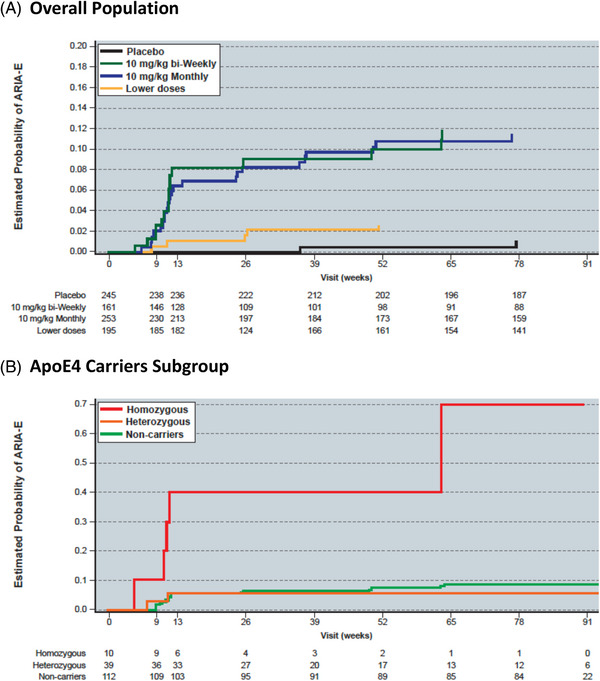
\includegraphics[
                        width=8cm,
                        trim={0 0 0 9.5cm},
                        clip
                    ]{data/aria_population.jpg}
                };
            }
            \visible<5>{
                \node[draw=black, inner sep=0pt] at (0, 0) {
                    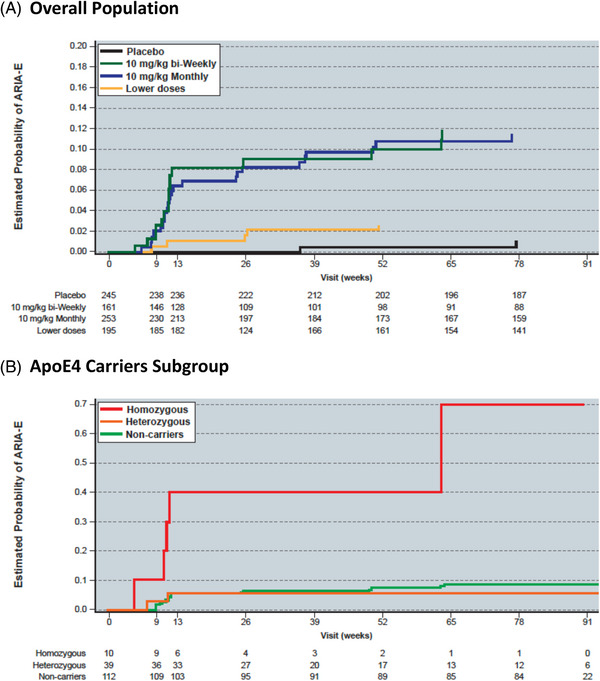
\includegraphics[
                        width=8cm,
                        trim={0 9cm 0 0},
                        clip
                    ]{data/aria_population.jpg}
                };
            }
            \visible<6,9>{
                \node[anchor=south, font=\tiny\linespread{0.9}\selectfont, text width=10.5cm, align=center] at (0, -4.15) {
                    Cummings, J., Apostolova, L., Rabinovici, G. D., Atri, A., Aisen, P., Greenberg, S., ... \& Salloway, S. (2023). Lecanemab: appropriate use recommendations. \textit{The journal of prevention of Alzheimer's disease}, \textit{10}(3), 362-377.
                };
            }
            \visible<6>{
                \node[text width=10cm, font=\scriptsize\linespread{0.9}\selectfont, align=flush left] at (0, 0) {
                    "MRI-based exclusion criteria of the lecanemab phase 3 (CLARITY AD) study included a history of any CNS macrohemorrhage >10 mm in diameter, more than 4 microhemorrhages (<10 mm in diameter), evidence of superficial siderosis, evidence of brain vasogenic edema, significant white matter hyperintensities, multiple lacunar strokes, or any cerebral strokes involving a major vascular territory. Evidence of cerebral contusion, encephalomalacia, brain aneurysms or other vascular malformations, central nervous system (CNS) infection, and brain tumors other than meningioma or arachnoid cysts excluded patients from phase 3 trial participation. \textbf{These same restrictions should apply when considering patients for treatment with lecanemab.} MRI evidence of underlying CAA-ri/ABRA or other conditions placing patients at risk for ARIA as well as more serious forms of ARIA should exclude patients as treatment candidates."
                };
            }
            \visible<7>{
                \node[anchor=east, text depth=0, font=\footnotesize] (x0) at (-1.8, 0.5) {
                    Imaging data
                };
                \node[anchor=east, text depth=0, font=\footnotesize] (x1) at (-1.8, 0) {
                    Clinical history
                };
                \node[anchor=east, text depth=0, font=\footnotesize] (x2) at (-1.8, -0.5) {
                    Cognitive tests
                };

                \node[draw=black, minimum height=2cm, minimum width=3cm, align=center, font=\normalfont\linespread{0.95}\selectfont, label=above:\footnotesize{Artificial neural network}] (model) at (0.3, 0) {};

                \nnneuron{(-0.8, 0.7)}{n00}{black!80}
                \nnneuron{(-0.8, 0.35)}{n01}{black!60}
                \nnneuron{(-0.8, 0)}{n02}{black!95}
                \nnneuron{(-0.8, -0.35)}{n03}{black!20}
                \nnneuron{(-0.8, -0.7)}{n04}{black!45}
                \nnneuron{(0.3, 0.35)}{n10}{black!52}
                \nnneuron{(0.3, 0)}{n11}{black!83}
                \nnneuron{(0.3, -0.35)}{n12}{black}
                \nnneuron{(1.4, 0)}{n20}{black!75}

                \node[anchor=west, text depth=0, font=\footnotesize] (y) at (2.4, 0) {
                    ARIA risk
                };

                \neuronconnection{x0}{n00}{gray}{-stealth}
                \neuronconnection{x0}{n01}{gray}{-stealth}
                \neuronconnection{x0}{n02}{gray}{-stealth}
                \neuronconnection{x0}{n03}{gray}{-stealth}
                \neuronconnection{x0}{n04}{gray}{-stealth}
                \neuronconnection{x1}{n00}{gray}{-stealth}
                \neuronconnection{x1}{n01}{gray}{-stealth}
                \neuronconnection{x1}{n02}{gray}{-stealth}
                \neuronconnection{x1}{n03}{gray}{-stealth}
                \neuronconnection{x1}{n04}{gray}{-stealth}
                \neuronconnection{x2}{n00}{gray}{-stealth}
                \neuronconnection{x2}{n01}{gray}{-stealth}
                \neuronconnection{x2}{n02}{gray}{-stealth}
                \neuronconnection{x2}{n03}{gray}{-stealth}
                \neuronconnection{x2}{n04}{gray}{-stealth}

                \neuronconnection{n00}{n10}{black!70}{-}
                \neuronconnection{n00}{n11}{black!32}{-}
                \neuronconnection{n00}{n12}{black!50}{-}
                \neuronconnection{n01}{n10}{black!65}{-}
                \neuronconnection{n01}{n11}{black!92}{-}
                \neuronconnection{n01}{n12}{black!50}{-}
                \neuronconnection{n02}{n10}{black!25}{-}
                \neuronconnection{n02}{n11}{black!67}{-}
                \neuronconnection{n02}{n12}{black!73}{-}
                \neuronconnection{n03}{n10}{black!42}{-}
                \neuronconnection{n03}{n11}{black!18}{-}
                \neuronconnection{n03}{n12}{black!23}{-}
                \neuronconnection{n04}{n10}{black!40}{-}
                \neuronconnection{n04}{n11}{black!62}{-}
                \neuronconnection{n04}{n12}{black!52}{-}

                \neuronconnection{n10}{n20}{black!52}{-}
                \neuronconnection{n11}{n20}{black!83}{-}
                \neuronconnection{n12}{n20}{black!70}{-}

                \neuronconnection{n20}{y}{gray}{-stealth}
            }
            \visible<8>{
                \node[] at (0, 0) {
                    \usebox{\responseprediction}
                };
            }
            \visible<9>{
                \node[text width=10cm, font=\scriptsize\linespread{0.9}\selectfont, align=flush left] at (0, 0) {
                    "We recommend obtaining MRIs after the \textbf{5th, 7th, and 14th infusions} as outlined in the PI. We recommend an additional week 52 (i.e., before the 26th infusion) MRI scan, especially for APOE4 carriers and those with evidence of ARIA on earlier MRIs."
                };
            }
            \visible<10>{
                \node[] at (0, 0) {
                    \usebox{\responsetrajectory}
                };
            }
            \visible<11>{
                \node[draw=black, inner sep=0pt] at (0, 0) {
                    \includegraphics[width=5cm]{data/icobrain_aria.png}
                };
            }
        \end{tikzpicture}
    \end{frame}

\end{document}
